\documentclass[aspectratio=169,table]{beamer}
\usepackage[utf8]{inputenc}
\usepackage[T1]{fontenc}
\usepackage{amsmath}
\usepackage{amssymb}
\usepackage{tikz}
\usepackage{circuitikz}
\usepackage{graphicx}
\usepackage{array}
\usepackage{multirow}

\usetheme{Madrid}
\usecolortheme{default}

% Definizione colori personalizzati
\definecolor{orangetheme}{RGB}{204,85,0}
\setbeamercolor{structure}{fg=orangetheme}
\setbeamercolor{frametitle}{bg=orangetheme,fg=white}
\setbeamercolor{title}{bg=orangetheme,fg=white}

% Rimuovi simboli di navigazione
\setbeamertemplate{navigation symbols}{}

% Numero di slide
\setbeamertemplate{footline}[frame number]

\title{Fondamenti di Informatica}
\subtitle{Algebra di Boole e Circuiti Logici}
\author{Prof. Fedeli Massimo}
\institute{IIS Fermi Sacconi Cpia\\}
\date{Tutti i diritti riservati}

\begin{document}

% Slide titolo
\begin{frame}
\titlepage
\end{frame}

% Slide 1: L'Algebra di Boole - 1/4
\begin{frame}{L'Algebra di Boole -- 1/4}
\begin{block}{Un po' di storia}
\begin{itemize}
\item Il matematico inglese \textbf{George Boole} nel 1847 fondò un campo della matematica e della filosofia chiamato \textbf{logica simbolica}
\item \textbf{Shannon} per primo applicò la logica simbolica ai circuiti nel 1939
\end{itemize}
\end{block}

\begin{block}{L'algebra di Boole è caratterizzata da}
\begin{itemize}
\item \textbf{Variabili booleane (o binarie):} variabili i cui valori possono essere 0 oppure 1
\begin{itemize}
\item Ma anche: vero/falso, on/off, sì/no
\end{itemize}
\item \textbf{Operazioni (o funzioni) booleane:} funzioni i cui input ed output sono variabili booleane
\end{itemize}
\end{block}
\end{frame}

% Slide 2: Relazione con i circuiti logici
\begin{frame}{L'Algebra di Boole -- 2/4}
\begin{block}{Relazione con i circuiti logici}
\begin{itemize}
\item Si studia l'algebra booleana poiché le sue funzioni sono \textbf{isomorfe} ai circuiti digitali: un circuito digitale può essere espresso tramite un'espressione booleana e viceversa
\item Le variabili booleane corrispondono a \textbf{segnali}
\item Le funzioni booleane corrispondono a \textbf{circuiti}
\end{itemize}
\end{block}

\vfill
\centering
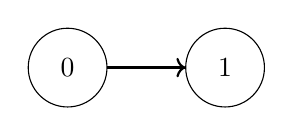
\begin{tikzpicture}
\node[draw, circle, minimum size=1cm] at (0,0) {0};
\node[draw, circle, minimum size=1cm] at (2,0) {1};
\draw[->, thick] (0.5,0) -- (1.5,0);
\end{tikzpicture}
\end{frame}

% Slide 3: L'Algebra di Boole - 3/4
\begin{frame}{L'Algebra di Boole -- 3/4}
\begin{itemize}
\item Come variabili contempla solo due costanti: \textbf{0} e \textbf{1} (falso e vero)
\begin{itemize}
\item Corrispondono a due stati che si escludono a vicenda
\item Possono descrivere lo stato di apertura o chiusura di un generico contatto o di un circuito a più contatti
\end{itemize}
\vspace{0.5cm}
\item Sulle variabili booleane si definiscono le funzioni (od operazioni) \textbf{AND, OR, NOT}
\begin{itemize}
\item Ed altre definite a partire da esse
\end{itemize}
\end{itemize}

\vfill
\centering
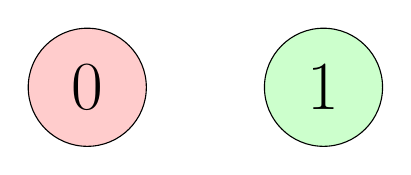
\begin{tikzpicture}
\node[draw, circle, fill=red!20, minimum size=1.5cm] at (0,0) {\Huge 0};
\node[draw, circle, fill=green!20, minimum size=1.5cm] at (3,0) {\Huge 1};
\end{tikzpicture}
\end{frame}

% Slide 4: L'Algebra di Boole - 4/4
\begin{frame}{L'Algebra di Boole -- 4/4}
\begin{itemize}
\item Le operazioni \textbf{AND} e \textbf{OR} sono operazioni \textbf{binarie} (agiscono su due operandi), l'operazione \textbf{NOT} è \textbf{unaria}
\vspace{0.5cm}
\item Nella valutazione delle espressioni booleane esiste una relazione di \textbf{precedenza} fra gli operatori NOT, AND e OR, nell'ordine in cui sono stati elencati
\begin{itemize}
\item Per alterare tale relazione bisogna usare le \textbf{parentesi}
\item Talvolta usate solo per maggiore chiarezza
\end{itemize}
\vspace{0.5cm}
\item Gli operatori dell'algebra booleana possono essere rappresentati e descritti in vari modi
\begin{itemize}
\item Spesso sono descritti semplicemente come AND, OR e NOT
\item Tavole di verità
\item Nella descrizione dei circuiti appaiono sotto forma di porte logiche
\end{itemize}
\end{itemize}
\end{frame}

% Slide 5: Operatore OR
\begin{frame}{Operatore (o funzione) OR}
\begin{block}{Somma logica (OR)}
Il valore della somma logica è il simbolo 1 se il valore di \textbf{almeno uno} degli operandi è il simbolo 1
\end{block}

\vspace{0.3cm}

\begin{columns}
\column{0.5\textwidth}
In generale, date $n$ variabili binarie, la loro somma logica (OR) è data da:
\[
x_1 + x_2 + \ldots + x_n = \begin{cases}
1 & \text{se almeno una } x_i \text{ vale 1} \\
0 & \text{se } x_1 = x_2 = \ldots = x_n = 0
\end{cases}
\]

\column{0.4\textwidth}
\centering
\textbf{Tavola di verità}

\begin{tabular}{|c|c|c|}
\hline
$x_1$ & $x_2$ & $F(x_1, x_2) = x_1 + x_2$ \\
\hline
0 & 0 & 0 \\
0 & 1 & 1 \\
1 & 0 & 1 \\
1 & 1 & 1 \\
\hline
\end{tabular}
\end{columns}
\end{frame}

% Slide 6: Operatore OR - Rappresentazioni
\begin{frame}{Operatore OR: Possibili Rappresentazioni}
\Large
\begin{itemize}
\item x $|$ y \hfill {\small $\leftarrow$ Usato in MATLAB}
\item or(x, y) \hfill {\small $\leftarrow$ Usato in MATLAB}
\item x \# y
\item x or y
\item x + y
\item $x \cup y$
\item $x \vee y$
\end{itemize}
\end{frame}

% Slide 7: Operatore AND
\begin{frame}{Operatore (o funzione) AND}
\begin{block}{Prodotto logico (AND)}
Il valore del prodotto logico è il simbolo 1 se il valore di \textbf{tutti} gli operandi è il simbolo 1
\end{block}

\vspace{0.3cm}

\begin{columns}
\column{0.5\textwidth}
In generale, date $n$ variabili binarie indipendenti, il loro prodotto logico (AND) è dato da:
\[
x_1 \cdot x_2 \cdot \ldots \cdot x_n = \begin{cases}
0 & \text{se almeno una } x_i \text{ vale 0} \\
1 & \text{se } x_1 = x_2 = \ldots = x_n = 1
\end{cases}
\]

\column{0.4\textwidth}
\centering
\textbf{Tavola di verità}

\begin{tabular}{|c|c|c|}
\hline
$x_1$ & $x_2$ & $F(x_1, x_2) = x_1 \times x_2$ \\
\hline
0 & 0 & 0 \\
0 & 1 & 0 \\
1 & 0 & 0 \\
1 & 1 & 1 \\
\hline
\end{tabular}
\end{columns}
\end{frame}

% Slide 8: Operatore AND - Rappresentazioni
\begin{frame}{Operatore AND: Possibili Rappresentazioni}
\Large
\begin{itemize}
\item x \& y \hfill {\small $\leftarrow$ Usato in MATLAB}
\item and(x, y) \hfill {\small $\leftarrow$ Usato in MATLAB}
\item x and y
\item $x \wedge y$
\item $x \cap y$
\item $x \times y$
\item x * y
\item xy
\end{itemize}
\end{frame}

% Slide 9: Operatore NOT
\begin{frame}{Operatore (o funzione) NOT}
\begin{block}{Operatore di negazione (NOT)}
Inverte il valore della costante su cui opera
\begin{itemize}
\item Noto anche come \textbf{inverter}
\end{itemize}
\end{block}

\vspace{0.3cm}

\begin{columns}
\column{0.5\textwidth}
In generale, la negazione di una variabile $x$ è:
\[
\bar{x} = \begin{cases}
0 & \text{se } x = 1 \\
1 & \text{se } x = 0
\end{cases}
\]

\vspace{0.3cm}
L'elemento $\bar{x} = \text{NOT}(x)$ viene detto \textbf{complemento} di $x$

Il complemento è unico

\column{0.4\textwidth}
\centering
\textbf{Proprietà}

\vspace{0.5cm}
$\bar{0} = 1$

$\bar{1} = 0$

$\overline{\bar{x}} = x$
\end{columns}
\end{frame}

% Slide 10: Operatore NOT - Rappresentazioni
\begin{frame}{Operatore NOT: Possibili Rappresentazioni}
\Large
\begin{itemize}
\item y = \textasciitilde x \hfill {\small $\leftarrow$ Usato in MATLAB}
\item y = not(x) \hfill {\small $\leftarrow$ Usato in MATLAB}
\item y = !x
\item y = not x
\item y = x'
\item y = $\neg x$
\item y = $\bar{x}$
\end{itemize}
\end{frame}

% Slide 11: Identità dell'Algebra di Boole
\begin{frame}{Algebra di Boole: Alcune Identità}
\small
\begin{columns}
\column{0.33\textwidth}
\centering
\textbf{Funzione AND}

\begin{align*}
0 \times 0 &= 0 \\
0 \times 1 &= 0 \\
1 \times 0 &= 0 \\
1 \times 1 &= 1 \\
x \times 0 &= 0 \\
0 \times x &= 0 \\
x \times 1 &= x \\
1 \times x &= x \\
\colorbox{yellow!30}{$x \times x = x$}
\end{align*}

\column{0.33\textwidth}
\centering
\textbf{Funzione OR}

\begin{align*}
0 + 0 &= 0 \\
0 + 1 &= 1 \\
1 + 0 &= 1 \\
1 + 1 &= 1 \\
x + 0 &= x \\
0 + x &= x \\
x + 1 &= 1 \\
1 + x &= 1 \\
\colorbox{yellow!30}{$x + x = x$}
\end{align*}

\column{0.33\textwidth}
\centering
\textbf{Funzione NOT}

\begin{align*}
x + \bar{x} &= 1 \\
x \times \bar{x} &= 0 \\
\overline{\bar{x}} &= x
\end{align*}

\vspace{1cm}
\textbf{Legge dell'idempotenza}
\end{columns}
\end{frame}

% Slide 12: Proprietà e Leggi
\begin{frame}{Algebra di Boole: Proprietà e Leggi}
\small
\begin{columns}
\column{0.48\textwidth}
\textbf{Proprietà Commutativa}
\begin{align*}
x_1 x_2 &= x_2 x_1 \\
x_1 + x_2 &= x_2 + x_1
\end{align*}

\textbf{Proprietà Distributiva}
\begin{align*}
x_1(x_2 + x_3) &= x_1 x_2 + x_1 x_3 \\
x_1 + x_2 x_3 &= (x_1 + x_2)(x_1 + x_3)
\end{align*}

\textbf{Proprietà Associativa}
\begin{align*}
x_1(x_2 x_3) &= (x_1 x_2)x_3 \\
x_1 + (x_2 + x_3) &= (x_1 + x_2) + x_3
\end{align*}

\column{0.48\textwidth}
\textbf{Leggi di Assorbimento}
\begin{align*}
x_1 + x_1 x_2 &= x_1 \\
x_1(x_1 + x_2) &= x_1
\end{align*}

\textbf{Leggi di De Morgan}
\begin{align*}
\overline{x_1 + x_2} &= \bar{x_1} \cdot \bar{x_2} \\
\overline{x_1 \cdot x_2} &= \bar{x_1} + \bar{x_2}
\end{align*}

\textbf{Altre Note}
\begin{align*}
x_1 + \bar{x_1} x_2 &= x_1 + x_2 \\
x_1(\bar{x_1} + x_2) &= x_1 x_2
\end{align*}
\end{columns}
\end{frame}

% Slide 13: Leggi di De Morgan - 1
\begin{frame}{Leggi di De Morgan -- 1/4}
\begin{block}{Prima Legge di De Morgan}
\[
\overline{x_1 + x_2} = \bar{x_1} \times \bar{x_2}
\]
\end{block}

\begin{itemize}
\item Il \textbf{complemento di una somma di variabili} è uguale al \textbf{prodotto dei complementi delle variabili}
\vspace{0.5cm}
\item Il complemento di due o più variabili poste in \textbf{OR} è uguale all'\textbf{AND} dei complementi delle singole variabili
\end{itemize}
\end{frame}

% Slide 14: Leggi di De Morgan - 2
\begin{frame}{Leggi di De Morgan -- 2/4}
\begin{block}{Seconda Legge di De Morgan}
\[
\overline{x_1 \times x_2} = \bar{x_1} + \bar{x_2}
\]
\end{block}

\begin{itemize}
\item Il \textbf{complemento di un prodotto di variabili} è uguale alla \textbf{somma dei complementi delle variabili}
\vspace{0.5cm}
\item Il complemento di due o più variabili poste in \textbf{AND} è equivalente all'\textbf{OR} dei complementi delle singole variabili
\end{itemize}
\end{frame}

% Slide 15: Leggi di De Morgan - 3
\begin{frame}{Leggi di De Morgan -- 3/4}
\begin{itemize}
\item Osservazione: $\overline{\bar{x}} = x$ \hfill (Eq. 1)
\vspace{0.3cm}
\item Legge 1 di De Morgan: $\overline{x_1 + x_2} = \bar{x_1} \times \bar{x_2}$ \hfill (Eq. 2)
\vspace{0.3cm}
\item Utilizzando (Eq. 1) posso scrivere (Eq. 2) come: $\overline{\overline{x_1 + x_2}} = \overline{\bar{x_1} \times \bar{x_2}}$
\vspace{0.3cm}
\item Utilizzando ancora (Eq. 1) ottengo: $x_1 + x_2 = \overline{\bar{x_1} \times \bar{x_2}}$
\end{itemize}

\vspace{0.5cm}
\begin{alertblock}{Conclusione}
L'\textbf{OR} fra $x_1$ e $x_2$ può essere espresso in termini delle sole operazioni \textbf{AND e NOT}
\begin{itemize}
\item Ogni espressione può essere espressa in termini delle sole due operazioni logiche AND e NOT
\end{itemize}
\end{alertblock}
\end{frame}

% Slide 16: Leggi di De Morgan - 4
\begin{frame}{Leggi di De Morgan -- 4/4}
\begin{itemize}
\item Osservazione: $\overline{\bar{x}} = x$ \hfill (Eq. 1)
\vspace{0.3cm}
\item Legge 2 di De Morgan: $\overline{x_1 \times x_2} = \bar{x_1} + \bar{x_2}$ \hfill (Eq. 3)
\vspace{0.3cm}
\item Utilizzando (Eq. 1) posso scrivere (Eq. 3) come: $\overline{\overline{x_1 \times x_2}} = \overline{\bar{x_1} + \bar{x_2}}$
\vspace{0.3cm}
\item Utilizzando ancora (Eq. 1) ottengo: $x_1 \times x_2 = \overline{\bar{x_1} + \bar{x_2}}$
\end{itemize}

\vspace{0.5cm}
\begin{alertblock}{Conclusione}
L'\textbf{AND} fra $x_1$ e $x_2$ può essere espresso in termini delle sole operazioni \textbf{OR e NOT}
\begin{itemize}
\item Ogni espressione può essere espressa in termini delle sole due operazioni logiche OR e NOT
\end{itemize}
\end{alertblock}
\end{frame}

% Slide 17: Osservazioni
\begin{frame}{Alcune Osservazioni}
\begin{itemize}
\item Identità, proprietà e leggi viste fino ad ora sono generalmente applicate nelle \textbf{trasformazioni di funzioni booleane} in altre equivalenti, ma di più facile realizzazione circuitale
\vspace{1cm}
\item Dalle \textbf{leggi di De Morgan} si evince che la scelta delle funzioni OR, AND e NOT, come funzioni primitive, è \textbf{ridondante}
\end{itemize}
\end{frame}

% Slide 18: Funzioni Logiche - 1
\begin{frame}{Funzioni Logiche (o Booleane) -- 1/5}
\begin{columns}
\column{0.55\textwidth}
\begin{itemize}
\item Date $n$ variabili booleane indipendenti $x_1, x_2, \ldots, x_n$, queste possono assumere $2^n$ configurazioni distinte
\vspace{0.3cm}
\item Ad esempio per $n = 3$ si hanno 8 configurazioni
\vspace{0.3cm}
\item Ogni riga mostra il valore restituito a partire da una particolare configurazione dell'input
\vspace{0.3cm}
\item Una configurazione specifica è individuata univocamente da un AND di tutte le variabili, dove quelle corrispondenti ai valori 0 compaiono negate
\begin{itemize}
\item \textbf{Prodotto fondamentale} o \textbf{prodotto minimo} (minterm)
\end{itemize}
\end{itemize}

\column{0.4\textwidth}
\centering
\begin{tabular}{|c|c|c|c|}
\hline
$x_1$ & $x_2$ & $x_3$ & $F$ \\
\hline
0 & 0 & 0 & 0 \\
0 & 0 & 1 & 0 \\
0 & 1 & 0 & 0 \\
\rowcolor{red!20}
0 & 1 & 1 & 1 \\
1 & 0 & 0 & 0 \\
1 & 0 & 1 & 1 \\
1 & 1 & 0 & 1 \\
1 & 1 & 1 & 1 \\
\hline
\end{tabular}

\vspace{0.3cm}
$x_1 x_2 x_3 \rightarrow 010$
\end{columns}
\end{frame}

% Slide 19: Funzioni Logiche - 2
\begin{frame}{Funzioni Logiche (o Booleane) -- 2/5}
\begin{columns}
\column{0.45\textwidth}
\small
\begin{tabular}{|c|c|c|c|}
\hline
$x_1$ & $x_2$ & $x_3$ & $F$ \\
\hline
0 & 0 & 0 & 0 \\
0 & 0 & 1 & 0 \\
0 & 1 & 0 & 0 \\
0 & 1 & 1 & 1 \\
1 & 0 & 0 & 0 \\
1 & 0 & 1 & 1 \\
1 & 1 & 0 & 1 \\
1 & 1 & 1 & 1 \\
\hline
\end{tabular}

\column{0.5\textwidth}
\textbf{Configurazioni}

\small
\begin{align*}
000 &\rightarrow \bar{x_1} \bar{x_2} \bar{x_3} \\
001 &\rightarrow \bar{x_1} \bar{x_2} x_3 \\
010 &\rightarrow \bar{x_1} x_2 \bar{x_3} \\
011 &\rightarrow \bar{x_1} x_2 x_3 \\
100 &\rightarrow x_1 \bar{x_2} \bar{x_3} \\
101 &\rightarrow x_1 \bar{x_2} x_3 \\
110 &\rightarrow x_1 x_2 \bar{x_3} \\
111 &\rightarrow x_1 x_2 x_3
\end{align*}
\end{columns}

\vspace{0.5cm}
\begin{itemize}
\item Se in una configurazione una variabile compare con 1, si assume il valore diretto
\item Se compare con 0, si assume il valore negato
\end{itemize}
\end{frame}

% Slide 20: Funzioni Logiche - 3
\begin{frame}{Funzioni Logiche (o Booleane) -- 3/5}
\begin{block}{Definizione di Funzione Booleana}
Una variabile $y$ è \textbf{funzione} delle $n$ variabili indipendenti $x_1, x_2, \ldots, x_n$, quando esiste un criterio che fa corrispondere in modo univoco ad ognuna delle $2^n$ configurazioni di $x$ un determinato valore $y$ (ovviamente 0 o 1)
\end{block}

\[
y = F(x_1, x_2, \ldots, x_n)
\]

\vspace{0.3cm}

\begin{columns}
\column{0.5\textwidth}
Una rappresentazione esplicita di una funzione è la \textbf{tavola di verità}, in cui si elencano tutte le possibili combinazioni di $x_1, x_2, \ldots, x_n$, con associato il valore di $y$

\column{0.35\textwidth}
\centering
\begin{tabular}{|c|c|c|}
\hline
$x_1$ & $x_2$ & $y$ \\
\hline
0 & 0 & 0 \\
0 & 1 & 1 \\
1 & 0 & 1 \\
1 & 1 & 1 \\
\hline
\end{tabular}

\vspace{0.2cm}
$y = x_1 + x_2$
\end{columns}
\end{frame}

% Slide 21: Funzioni Logiche - 4
\begin{frame}{Funzioni Logiche (o Booleane) -- 4/5}
\small
\begin{columns}
\column{0.4\textwidth}
\begin{tabular}{|c|c|c|c|}
\hline
$x_1$ & $x_2$ & $x_3$ & $F$ \\
\hline
0 & 0 & 0 & 0 \\
0 & 0 & 1 & 0 \\
0 & 1 & 0 & 0 \\
\rowcolor{green!20}
0 & 1 & 1 & 1 \\
1 & 0 & 0 & 0 \\
\rowcolor{green!20}
1 & 0 & 1 & 1 \\
\rowcolor{green!20}
1 & 1 & 0 & 1 \\
\rowcolor{green!20}
1 & 1 & 1 & 1 \\
\hline
\end{tabular}

\column{0.58\textwidth}
\textbf{Procedimento:}
\begin{enumerate}
\item Identificare tutte le righe della tavola di verità che danno 1 in output
\item Per ogni riga con un 1 in output, scrivere la configurazione delle variabili che la definiscono
\item Collegare tramite OR tutte le configurazioni ottenute
\end{enumerate}

\vspace{0.3cm}
\[
F = \bar{x_1} x_2 x_3 + x_1 \bar{x_2} x_3 + x_1 x_2 \bar{x_3} + x_1 x_2 x_3
\]
\end{columns}
\end{frame}

% Slide 22: Funzioni Logiche - 5
\begin{frame}{Funzioni Logiche (o Booleane) -- 5/5}
\[
F(x_1, x_2, x_3) = \bar{x_1} x_2 x_3 + x_1 \bar{x_2} x_3 + x_1 x_2 \bar{x_3} + x_1 x_2 x_3
\]

\begin{block}{Forma Canonica}
Con l'uso dei \textbf{minterm} possiamo determinare l'espressione algebrica di una funzione booleana a partire dalla tavola di verità

L'espressione algebrica trovata si chiama \textbf{forma canonica} della funzione e si ottiene con uno sviluppo in minterm
\begin{itemize}
\item Una \textbf{somma (OR) di prodotti (AND)}
\end{itemize}
\end{block}

\vspace{0.3cm}
\begin{alertblock}{Proprietà}
Se un minterm assume valore 1, anche la funzione $F$ assume il valore 1
\end{alertblock}
\end{frame}

% Slide 23: Esempio XOR - 1
\begin{frame}{Esempio 1: la Funzione Exclusive OR (XOR) -- 1/2}
\begin{block}{Comportamento della funzione XOR}
$F =$ ``L'output deve essere 1 (vero) se \textbf{solo uno} dei suoi input è 1, ma \textbf{non} se entrambi gli input sono 1''
\end{block}

\vspace{0.5cm}

Questo può essere rifrasato come:

\begin{block}{}
$F =$ ``L'output è 1 se $(x_1$ OR $x_2)$ è 1, AND se $(x_1$ AND $x_2)$ sono NOT 1 (falso)''
\end{block}

\vspace{0.5cm}

Che può essere scritto come:
\[
F = (x_1 + x_2) \times \overline{(x_1 x_2)}
\]
\end{frame}

% Slide 24: Esempio XOR - 2
\begin{frame}{Esempio 1: la Funzione Exclusive OR (XOR) -- 2/2}
\begin{columns}
\column{0.4\textwidth}
La funzione XOR verifica la \textbf{disuguaglianza} di due variabili

\vspace{1cm}

\begin{tabular}{|c|c|c|}
\hline
$x_1$ & $x_2$ & XOR \\
\hline
0 & 0 & 0 \\
\rowcolor{yellow!30}
0 & 1 & 1 \\
\rowcolor{yellow!30}
1 & 0 & 1 \\
1 & 1 & 0 \\
\hline
\end{tabular}

\column{0.55\textwidth}
L'espressione come \textbf{somma di prodotti} è:
\[
\text{XOR}(x_1, x_2) = \bar{x_1} \times x_2 + x_1 \times \bar{x_2}
\]

\vspace{0.5cm}
\begin{alertblock}{Forma canonica}
Somma di prodotti (OR di AND)

\textbf{N.B.} tutte le funzioni logiche si possono scrivere in questa forma
\end{alertblock}
\end{columns}
\end{frame}

% Slide 25: Esempio 2
\begin{frame}{Esempio 2: dalla Tavola di Verità alla Funzione}
\begin{columns}
\column{0.4\textwidth}
\textbf{Problema:} date tre variabili booleane $(x, y, z)$, si scriva la funzione $F$ che vale 1 quando \textbf{solo due} di esse hanno valore 1

\vspace{0.5cm}

\begin{tabular}{|c|c|c|c|}
\hline
$x$ & $y$ & $z$ & $F$ \\
\hline
0 & 0 & 0 & 0 \\
0 & 0 & 1 & 0 \\
0 & 1 & 0 & 0 \\
\rowcolor{yellow!30}
0 & 1 & 1 & 1 \\
1 & 0 & 0 & 0 \\
\rowcolor{yellow!30}
1 & 0 & 1 & 1 \\
\rowcolor{yellow!30}
1 & 1 & 0 & 1 \\
1 & 1 & 1 & 0 \\
\hline
\end{tabular}

\column{0.55\textwidth}
\[
F(x, y, z) = \bar{x} y z + x \bar{y} z + x y \bar{z}
\]

\vspace{0.5cm}
\begin{block}{Forma canonica}
Somma di prodotti (OR di AND)

\textbf{N.B.} tutte le funzioni logiche si possono scrivere in questa forma
\end{block}
\end{columns}
\end{frame}

% Slide 26: Esempio 3
\begin{frame}{Esempio 3: dalla Tavola di Verità alla Funzione}
\begin{columns}
\column{0.4\textwidth}
\textbf{Problema:} date tre variabili booleane $(x, y, z)$, si scriva la funzione $F$ che vale 1 quando il \textbf{numero di 1 è dispari}

\vspace{0.5cm}

\begin{tabular}{|c|c|c|c|}
\hline
$x$ & $y$ & $z$ & $F$ \\
\hline
0 & 0 & 0 & 0 \\
\rowcolor{yellow!30}
0 & 0 & 1 & 1 \\
\rowcolor{yellow!30}
0 & 1 & 0 & 1 \\
0 & 1 & 1 & 0 \\
\rowcolor{yellow!30}
1 & 0 & 0 & 1 \\
1 & 0 & 1 & 0 \\
1 & 1 & 0 & 0 \\
\rowcolor{yellow!30}
1 & 1 & 1 & 1 \\
\hline
\end{tabular}

\column{0.55\textwidth}
\[
F(x, y, z) = \bar{x} \bar{y} z + \bar{x} y \bar{z} + x \bar{y} \bar{z} + x y z
\]

\vspace{0.5cm}
\begin{block}{Forma canonica}
Somma di prodotti (OR di AND)

\textbf{N.B.} tutte le funzioni logiche si possono scrivere in questa forma
\end{block}
\end{columns}
\end{frame}

% Slide 27: Esempio 4
\begin{frame}{Esempio 4: dalla Funzione alla Tavola di Verità}
\begin{columns}
\column{0.5\textwidth}
Vediamo un esempio per la funzione:
\[
F = x \times (\bar{y} + z)
\]

\vspace{1cm}

Per ogni combinazione di input:
\begin{itemize}
\item Calcolare $\bar{y}$
\item Calcolare $\bar{y} + z$
\item Calcolare $x \times (\bar{y} + z)$
\end{itemize}

\column{0.4\textwidth}
\centering
\begin{tabular}{|c|c|c|c|}
\hline
$x$ & $y$ & $z$ & $F$ \\
\hline
0 & 0 & 0 & 0 \\
0 & 0 & 1 & 0 \\
0 & 1 & 0 & 0 \\
0 & 1 & 1 & 0 \\
\rowcolor{green!20}
1 & 0 & 0 & 1 \\
1 & 0 & 1 & 0 \\
1 & 1 & 0 & 0 \\
1 & 1 & 1 & 0 \\
\hline
\end{tabular}
\end{columns}
\end{frame}

% Slide 28: Mappe di Karnaugh - 1
\begin{frame}{Le mappe di Karnaugh (1/2)}
Le \textbf{mappe di Karnaugh} sono un mezzo visivo per poter manipolare e semplificare le forme algebriche di una funzione.

\vspace{0.5cm}

\begin{columns}
\column{0.5\textwidth}
Per le funzioni fino a 4 variabili, i rispettivi termini sono disposti su una mappa in forma tabellare, e viene posto:
\begin{itemize}
\item \textbf{1} in corrispondenza del termine in cui la funzione assume valore 1
\item \textbf{0} altrimenti
\end{itemize}

\column{0.45\textwidth}
\textbf{Esempio: funzione XOR}

\begin{tabular}{|c|c|c|}
\hline
$x_1$ & $x_2$ & XOR \\
\hline
0 & 0 & 0 \\
0 & 1 & 1 \\
1 & 0 & 1 \\
1 & 1 & 0 \\
\hline
\end{tabular}

\vspace{0.5cm}

\begin{tabular}{c|c|c|}
\multicolumn{1}{c}{} & \multicolumn{1}{c}{0} & \multicolumn{1}{c}{1} \\
\cline{2-3}
0 & 0 & 1 \\
\cline{2-3}
1 & 1 & 0 \\
\cline{2-3}
\end{tabular}
\end{columns}
\end{frame}

% Slide 29: Mappe di Karnaugh - 2
\begin{frame}{Le mappe di Karnaugh (2/2)}
\small
\begin{columns}
\column{0.45\textwidth}
\textbf{Esempio con 4 variabili}

\begin{tabular}{|c|c|c|c|c|}
\hline
$x_1$ & $x_2$ & $x_3$ & $x_4$ & $f$ \\
\hline
0 & 0 & 0 & 0 & 1 \\
0 & 0 & 0 & 1 & 1 \\
0 & 0 & 1 & 0 & 1 \\
0 & 0 & 1 & 1 & 0 \\
0 & 1 & 0 & 0 & 0 \\
0 & 1 & 0 & 1 & 1 \\
\multicolumn{5}{c}{...} \\
\hline
\end{tabular}

\column{0.5\textwidth}
\textbf{Mappa di Karnaugh corrispondente}

\vspace{0.3cm}

\begin{tabular}{cc|c|c|c|c|}
\multicolumn{2}{c}{} & \multicolumn{4}{c}{$x_3 x_4$} \\
\multicolumn{2}{c}{} & 00 & 01 & 11 & 10 \\
\cline{3-6}
\multirow{4}{*}{\rotatebox{90}{$x_1 x_2$}} & 00 & 1 & 1 & 0 & 1 \\
\cline{3-6}
& 01 & 0 & 1 & 1 & 0 \\
\cline{3-6}
& 11 & 0 & 0 & 1 & 1 \\
\cline{3-6}
& 10 & 1 & 0 & 1 & 1 \\
\cline{3-6}
\end{tabular}
\end{columns}

\vspace{0.5cm}

\begin{block}{Proprietà importante}
Nelle mappe di Karnaugh si considerano \textbf{adiacenti} i quadratini che hanno un lato in comune e quelli posti alle \textbf{estremità opposte} della mappa
\end{block}
\end{frame}

% Slide 30: Mappe di Karnaugh - Semplificazione
\begin{frame}{Le mappe di Karnaugh -- Semplificazione}
\small
Le mappe consentono di semplificare la rappresentazione in forma canonica di una funzione booleana.

\vspace{0.3cm}

\begin{columns}
\column{0.35\textwidth}
\begin{tabular}{cc|c|c|c|c|}
\multicolumn{2}{c}{} & \multicolumn{4}{c}{$x_3 x_4$} \\
\multicolumn{2}{c}{} & 00 & 01 & 11 & 10 \\
\cline{3-6}
\multirow{4}{*}{\rotatebox{90}{$x_1 x_2$}} & 00 & \cellcolor{blue!20}1 & \cellcolor{blue!20}1 & 0 & \cellcolor{yellow!30}1 \\
\cline{3-6}
& 01 & 0 & \cellcolor{green!20}1 & \cellcolor{green!20}1 & 0 \\
\cline{3-6}
& 11 & 0 & 0 & \cellcolor{red!20}1 & \cellcolor{red!20}1 \\
\cline{3-6}
& 10 & \cellcolor{yellow!30}1 & 0 & \cellcolor{red!20}1 & \cellcolor{red!20}1 \\
\cline{3-6}
\end{tabular}

\column{0.6\textwidth}
\textbf{Procedimento:}
\begin{enumerate}
\item Identificare le celle adiacenti con valore 1
\item Rappresentare i termini caratterizzanti le celle così identificate
\end{enumerate}

\vspace{0.5cm}

\textbf{Espressione semplificata:}
\begin{align*}
f(x_1, x_2, x_3, x_4) = &\bar{x_1} \bar{x_2} \bar{x_3} + \\
&x_2 x_3 x_4 + \\
&x_3 x_4 + \\
&\bar{x_2} x_4
\end{align*}
\end{columns}
\end{frame}

% Slide 31: Circuiti Logici
\begin{frame}{Circuito Logico}
\begin{block}{Definizione}
Il cuore di un sistema digitale è il \textbf{circuito logico digitale}
\begin{itemize}
\item Progettato a partire da \textbf{porte logiche}
\item Collegate tra loro per formare circuiti più grandi
\item Combinati per realizzare circuiti di grande importanza pratica nell'architettura del computer
\end{itemize}
\end{block}

\vspace{0.5cm}

\centering
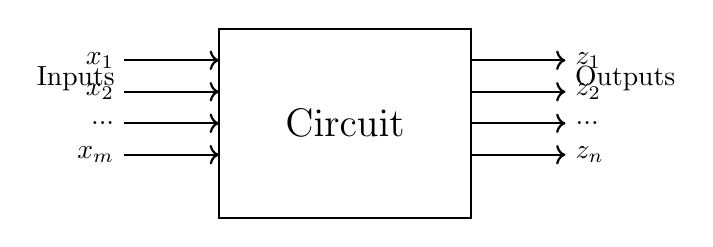
\begin{tikzpicture}[scale=0.8]
\draw[thick] (0,0) rectangle (4,3);
\node at (2,1.5) {\Large Circuit};

\draw[thick, <-] (0,2.5) -- (-1.5,2.5) node[left] {$x_1$};
\draw[thick, <-] (0,2) -- (-1.5,2) node[left] {$x_2$};
\draw[thick, <-] (0,1.5) -- (-1.5,1.5) node[left] {...};
\draw[thick, <-] (0,1) -- (-1.5,1) node[left] {$x_m$};
\node[left] at (-1.5,2.2) {Inputs};

\draw[thick, ->] (4,2.5) -- (5.5,2.5) node[right] {$z_1$};
\draw[thick, ->] (4,2) -- (5.5,2) node[right] {$z_2$};
\draw[thick, ->] (4,1.5) -- (5.5,1.5) node[right] {...};
\draw[thick, ->] (4,1) -- (5.5,1) node[right] {$z_n$};
\node[right] at (5.5,2.2) {Outputs};
\end{tikzpicture}
\end{frame}

% Slide 32: Porte Logiche
\begin{frame}{Porte Logiche}
\begin{itemize}
\item \textbf{Building block} utilizzati per creare circuiti digitali
\vspace{0.3cm}
\item Qualsiasi circuito può essere implementato usando solo porte logiche elementari (AND, OR e NOT)
\begin{itemize}
\item Le cose si fanno complicate quando si hanno numerosi input ed output
\end{itemize}
\vspace{0.3cm}
\item Dispositivi elettronici che implementano semplici funzioni booleane
\vspace{0.3cm}
\item Ciascuna porta ha il proprio \textbf{simbolo logico} che permette a funzioni complesse di essere rappresentate mediante un diagramma logico
\vspace{0.3cm}
\item La funzione di ciascuna porta può essere rappresentata da una \textbf{tavola di verità} o utilizzando la \textbf{notazione booleana}
\end{itemize}
\end{frame}

% Slide 33: Porta OR
\begin{frame}{Funzione OR: Tavola di Verità e Porta Logica}
\begin{columns}
\column{0.4\textwidth}
\centering
\textbf{Tavola di verità}

\vspace{0.5cm}

\begin{tabular}{|c|c|c|}
\hline
$x_1$ & $x_2$ & $x_1$ OR $x_2$ \\
\hline
0 & 0 & 0 \\
0 & 1 & 1 \\
1 & 0 & 1 \\
1 & 1 & 1 \\
\hline
\end{tabular}

\column{0.5\textwidth}
\centering
\textbf{Porta logica}

\vspace{0.5cm}

\begin{circuitikz}[scale=1.2]
\draw (0,0) node[or port] (or) {};
\draw (or.in 1) node[left] {$x_1$};
\draw (or.in 2) node[left] {$x_2$};
\draw (or.out) node[right] {$x_1 + x_2$};
\end{circuitikz}
\end{columns}
\end{frame}

% Slide 34: Porta AND
\begin{frame}{Funzione AND: Tavola di Verità e Porta Logica}
\begin{columns}
\column{0.4\textwidth}
\centering
\textbf{Tavola di verità}

\vspace{0.5cm}

\begin{tabular}{|c|c|c|}
\hline
$x_1$ & $x_2$ & $x_1$ AND $x_2$ \\
\hline
0 & 0 & 0 \\
0 & 1 & 0 \\
1 & 0 & 0 \\
1 & 1 & 1 \\
\hline
\end{tabular}

\column{0.5\textwidth}
\centering
\textbf{Porta logica}

\vspace{0.5cm}

\begin{circuitikz}[scale=1.2]
\draw (0,0) node[and port] (and) {};
\draw (and.in 1) node[left] {$x_1$};
\draw (and.in 2) node[left] {$x_2$};
\draw (and.out) node[right] {$x_1 \cdot x_2$};
\end{circuitikz}
\end{columns}
\end{frame}

% Slide 35: Porta NOT
\begin{frame}{Funzione NOT: Tavola di Verità e Porta Logica}
\begin{columns}
\column{0.4\textwidth}
\centering
\textbf{Tavola di verità}

\vspace{0.5cm}

\begin{tabular}{|c|c|}
\hline
$x$ & NOT $x$ \\
\hline
0 & 1 \\
1 & 0 \\
\hline
\end{tabular}

\column{0.5\textwidth}
\centering
\textbf{Porta logica}

\vspace{0.5cm}

\begin{circuitikz}[scale=1.2]
\draw (0,0) node[not port] (not) {};
\draw (not.in) node[left] {$x$};
\draw (not.out) node[right] {$\bar{x}$};
\end{circuitikz}
\end{columns}
\end{frame}

% Slide 36: Porta NAND
\begin{frame}{Porta NAND}
\centering
\begin{columns}
\column{0.3\textwidth}
\textbf{(a) Circuit symbol}

\vspace{0.5cm}

\begin{circuitikz}[scale=1.5]
\draw (0,0) node[nand port] (nand) {};
\draw (nand.in 1) node[left] {A};
\draw (nand.in 2) node[left] {B};
\draw (nand.out) node[right] {C};
\end{circuitikz}

\column{0.3\textwidth}
\textbf{(b) Truth table}

\vspace{0.5cm}

\begin{tabular}{|c|c|c|}
\hline
A & B & C \\
\hline
0 & 0 & 1 \\
0 & 1 & 1 \\
1 & 0 & 1 \\
1 & 1 & 0 \\
\hline
\end{tabular}

\column{0.35\textwidth}
\textbf{(c) Boolean expression}

\vspace{0.5cm}

\[
C = \overline{A \cdot B}
\]
\end{columns}
\end{frame}

% Slide 37: Porta NOR
\begin{frame}{Porta NOR}
\centering
\begin{columns}
\column{0.3\textwidth}
\textbf{(a) Circuit symbol}

\vspace{0.5cm}

\begin{circuitikz}[scale=1.5]
\draw (0,0) node[nor port] (nor) {};
\draw (nor.in 1) node[left] {A};
\draw (nor.in 2) node[left] {B};
\draw (nor.out) node[right] {C};
\end{circuitikz}

\column{0.3\textwidth}
\textbf{(b) Truth table}

\vspace{0.5cm}

\begin{tabular}{|c|c|c|}
\hline
A & B & C \\
\hline
0 & 0 & 1 \\
0 & 1 & 0 \\
1 & 0 & 0 \\
1 & 1 & 0 \\
\hline
\end{tabular}

\column{0.35\textwidth}
\textbf{(c) Boolean expression}

\vspace{0.5cm}

\[
C = \overline{A + B}
\]
\end{columns}
\end{frame}

% Slide 38: Porta XOR
\begin{frame}{Porta XOR}
\centering
\begin{columns}
\column{0.3\textwidth}
\textbf{(a) Circuit symbol}

\vspace{0.5cm}

\begin{circuitikz}[scale=1.5]
\draw (0,0) node[xor port] (xor) {};
\draw (xor.in 1) node[left] {A};
\draw (xor.in 2) node[left] {B};
\draw (xor.out) node[right] {C};
\end{circuitikz}

\column{0.3\textwidth}
\textbf{(b) Truth table}

\vspace{0.5cm}

\begin{tabular}{|c|c|c|}
\hline
A & B & C \\
\hline
0 & 0 & 0 \\
0 & 1 & 1 \\
1 & 0 & 1 \\
1 & 1 & 0 \\
\hline
\end{tabular}

\column{0.35\textwidth}
\textbf{(c) Boolean expression}

\vspace{0.5cm}

\[
C = A \oplus B
\]
\end{columns}
\end{frame}

% Slide 39: Porta XNOR
\begin{frame}{Porta Exclusive NOR}
\centering
\begin{columns}
\column{0.3\textwidth}
\textbf{(a) Circuit symbol}

\vspace{0.5cm}

\begin{circuitikz}[scale=1.5]
\draw (0,0) node[xnor port] (xnor) {};
\draw (xnor.in 1) node[left] {A};
\draw (xnor.in 2) node[left] {B};
\draw (xnor.out) node[right] {C};
\end{circuitikz}

\column{0.3\textwidth}
\textbf{(b) Truth table}

\vspace{0.5cm}

\begin{tabular}{|c|c|c|}
\hline
A & B & C \\
\hline
0 & 0 & 1 \\
0 & 1 & 0 \\
1 & 0 & 0 \\
1 & 1 & 1 \\
\hline
\end{tabular}

\column{0.35\textwidth}
\textbf{(c) Boolean expression}

\vspace{0.5cm}

\[
C = \overline{A \oplus B}
\]
\end{columns}
\end{frame}

% Slide 40: Esempio 5 - dalla funzione al circuito
\begin{frame}{Esempio 5: dalla Funzione al Circuito}
\[
X = A + B\bar{C}
\]

\vspace{1cm}

\centering
\begin{circuitikz}[scale=0.9]
% Input A diretto a OR
\draw (0,3) node[left] {A} -- (5,3);

% Input B
\draw (0,1.5) node[left] {B} -- (2,1.5);

% Input C -> NOT -> AND con B
\draw (0,0) node[left] {C} -- (1,0);
\draw (1,0) node[not port, anchor=in] (not1) {};
\draw (not1.out) -- (2,0) node[anchor=south] {$\bar{C}$};

% AND tra B e C negato
\draw (2,0.75) node[and port, anchor=in 2, number inputs=2] (and1) {};
\draw (2,1.5) -- (and1.in 1);
\draw (2,0) -- (and1.in 2);
\draw (and1.out) -- (4,0.75) node[anchor=south] {$B\bar{C}$};

% OR finale
\draw (5,1.875) node[or port, anchor=in 1, number inputs=2] (or1) {};
\draw (5,3) -- (or1.in 1);
\draw (4,0.75) -- (4,1.875) -- (or1.in 2);
\draw (or1.out) -- (6.5,1.875) node[right] {$X = A + B\bar{C}$};
\end{circuitikz}
\end{frame}

% Slide 41: Esempio 6 - dalla funzione al circuito
\begin{frame}{Esempio 6: dalla Funzione al Circuito}
\[
C = (A + B) \cdot \overline{(AB)}
\]

\vspace{0.5cm}

\begin{columns}
\column{0.4\textwidth}
\small
\begin{tabular}{|c|c|c|}
\hline
A & B & C \\
\hline
0 & 0 & 1 \\
0 & 1 & 1 \\
1 & 0 & 1 \\
1 & 1 & 0 \\
\hline
\end{tabular}

\vspace{0.3cm}
\textbf{Porta NAND}

\column{0.55\textwidth}
\begin{circuitikz}[scale=0.7]
% Inputs
\draw (0,3) node[left] {A} -- (1,3);
\draw (0,1.5) node[left] {B} -- (1,1.5);

% OR superiore
\draw (1.5,2.625) node[or port, number inputs=2] (or1) {};
\draw (1,3) |- (or1.in 1);
\draw (1,1.5) |- (or1.in 2);
\draw (or1.out) -- (3.5,2.625) node[anchor=south] {$A+B$};

% NAND inferiore
\draw (1.5,0.75) node[nand port, number inputs=2] (nand1) {};
\draw (1,3) |- (nand1.in 1);
\draw (1,1.5) |- (nand1.in 2);
\draw (nand1.out) -- (3.5,0.75) node[anchor=north] {$\overline{AB}$};

% AND finale
\draw (4.5,1.6875) node[and port, number inputs=2] (and1) {};
\draw (3.5,2.625) -| (and1.in 1);
\draw (3.5,0.75) -| (and1.in 2);
\draw (and1.out) -- (6,1.6875) node[right] {$C=(A+B)\cdot\overline{AB}$};
\end{circuitikz}
\end{columns}
\end{frame}

% Slide 42: Esempio 7
\begin{frame}{Esempio 7: dalla Funzione al Circuito}
\[
X = \bar{A}BC + A\bar{B}C + AB\bar{C}
\]

\vspace{0.5cm}

\centering
\begin{circuitikz}[scale=0.65, transform shape]
% Inputs e NOT
\draw (0,6) node[left] {A} -- (1,6);
\draw (1,6) node[not port, anchor=in] (notA) {};
\draw (notA.out) -- (2,6) node[anchor=south] {$\bar{A}$};

\draw (0,4) node[left] {B} -- (1,4);
\draw (1,4) node[not port, anchor=in] (notB) {};
\draw (notB.out) -- (2,4) node[anchor=south] {$\bar{B}$};

\draw (0,2) node[left] {C} -- (1,2);
\draw (1,2) node[not port, anchor=in] (notC) {};
\draw (notC.out) -- (2,2) node[anchor=south] {$\bar{C}$};

% AND gates
\draw (3.5,5.5) node[and port, number inputs=3] (and1) {};
\draw (2,6) |- (and1.in 1);
\draw (0,4) -- (3,4) |- (and1.in 2);
\draw (0,2) -- (2.5,2) |- (and1.in 3);
\draw (and1.out) -- (5.5,5.5) node[anchor=south] {$\bar{A}BC$};

\draw (3.5,3.5) node[and port, number inputs=3] (and2) {};
\draw (0,6) -- (2.8,6) |- (and2.in 1);
\draw (2,4) |- (and2.in 2);
\draw (0,2) -- (2.3,2) |- (and2.in 3);
\draw (and2.out) -- (5.5,3.5) node[anchor=south] {$A\bar{B}C$};

\draw (3.5,1.5) node[and port, number inputs=3] (and3) {};
\draw (0,6) -- (2.6,6) |- (and3.in 1);
\draw (0,4) -- (2.7,4) |- (and3.in 2);
\draw (2,2) |- (and3.in 3);
\draw (and3.out) -- (5.5,1.5) node[anchor=south] {$AB\bar{C}$};

% OR finale
\draw (7,3.5) node[or port, number inputs=3] (or1) {};
\draw (5.5,5.5) -| (or1.in 1);
\draw (5.5,3.5) -- (or1.in 2);
\draw (5.5,1.5) -| (or1.in 3);
\draw (or1.out) -- (9,3.5) node[right] {$X=\bar{A}BC+A\bar{B}C+AB\bar{C}$};
\end{circuitikz}
\end{frame}

% Slide 43: Esempio 8
\begin{frame}{Esempio 8: dalla Funzione al Circuito}
\[
Y = \overline{AB} + \overline{CD}
\]

\vspace{0.3cm}

\begin{columns}
\column{0.3\textwidth}
\small
\begin{tabular}{|c|c|c|}
\hline
A & B & C \\
\hline
0 & 0 & 1 \\
0 & 1 & 0 \\
1 & 0 & 0 \\
1 & 1 & 0 \\
\hline
\end{tabular}

\column{0.65\textwidth}
\begin{circuitikz}[scale=0.8]
% Input A -> NOT
\draw (0,3.5) node[left] {A} -- (1,3.5);
\draw (1,3.5) node[not port, anchor=in] (notA) {};
\draw (notA.out) -- (2,3.5) node[anchor=south] {$\bar{A}$};

% Input B
\draw (0,2.5) node[left] {B} -- (3,2.5);

% AND con A negato e B
\draw (3,3) node[and port, anchor=in 2, number inputs=2] (and1) {};
\draw (2,3.5) |- (and1.in 1);
\draw (3,2.5) -- (and1.in 2);
\draw (and1.out) -- (4.5,3) node[anchor=south] {$\overline{AB}$};

% Input C
\draw (0,1) node[left] {C} -- (3,1);

% Input D -> NOT
\draw (0,-0.5) node[left] {D} -- (1,-0.5);
\draw (1,-0.5) node[not port, anchor=in] (notD) {};
\draw (notD.out) -- (2,-0.5) node[anchor=north] {$\bar{D}$};

% AND con C e D negato
\draw (3,0.25) node[and port, anchor=in 2, number inputs=2] (and2) {};
\draw (3,1) -- (and2.in 1);
\draw (2,-0.5) |- (and2.in 2);
\draw (and2.out) -- (4.5,0.25) node[anchor=north] {$\overline{CD}$};

% NOR finale
\draw (5.5,1.625) node[nor port, number inputs=2] (nor1) {};
\draw (4.5,3) -| (nor1.in 1);
\draw (4.5,0.25) -| (nor1.in 2);
\draw (nor1.out) -- (7,1.625) node[right] {$Y=\overline{AB}+\overline{CD}$};

\node[red, draw, thick] at (5.5,1.625) {};
\node[red] at (5.5,-1) {Porta NOR};
\end{circuitikz}
\end{columns}
\end{frame}

% Slide 44: Esempio 9 - Dal circuito alla funzione
\begin{frame}{Esempio 9: dal Circuito alla Funzione -- 1/2}
\centering
\begin{circuitikz}[scale=1]
\draw (0,3) node[left] {A} -- (1,3);
\draw (1,3) node[not port, anchor=in, label={[label distance=0.1cm]above:1}] (not1) {};

\draw (0,1.5) node[left] {B} -- (2.5,1.5);

\draw (0,0) node[left] {C} -- (2.5,0);

% NAND superiore
\draw (3,2.25) node[nand port, anchor=in 2, number inputs=2, label={[label distance=0.1cm]above:2}] (nand1) {};
\draw (not1.out) |- (nand1.in 1);
\draw (2.5,1.5) -- (nand1.in 2);

% AND inferiore
\draw (3,0.75) node[and port, anchor=in 2, number inputs=2, label={[label distance=0.1cm]above:3}] (and1) {};
\draw (2.5,1.5) |- (and1.in 1);
\draw (2.5,0) -- (and1.in 2);

% NAND finale
\draw (5,1.5) node[nand port, anchor=in 2, number inputs=2, label={[label distance=0.1cm]above:4}] (nand2) {};
\draw (nand1.out) -- (nand2.in 1);
\draw (and1.out) -- (nand2.in 2);
\draw (nand2.out) -- (6.5,1.5) node[right] {Z};
\end{circuitikz}

\vspace{1cm}
\textbf{Procedere progressivamente dagli input verso l'output}
\end{frame}

% Slide 45: Esempio 9 - Dal circuito alla funzione - 2
\begin{frame}{Esempio 9: dal Circuito alla Funzione -- 2/2}
\centering
\begin{circuitikz}[scale=0.9]
\draw (0,3) node[left] {A} -- (1,3);
\draw (1,3) node[not port, anchor=in] (not1) {};
\draw (not1.out) -- (2,3) node[anchor=south] {$\bar{A}$};

\draw (0,1.5) node[left] {B} -- (2.5,1.5);

\draw (0,0) node[left] {C} -- (2.5,0);

% NAND superiore
\draw (3,2.25) node[nand port, anchor=in 2, number inputs=2] (nand1) {};
\draw (2,3) |- (nand1.in 1);
\draw (2.5,1.5) -- (nand1.in 2);
\draw (nand1.out) -- (4.5,2.25) node[anchor=south] {$\overline{\bar{A}+B}$};

% AND inferiore
\draw (3,0.75) node[and port, anchor=in 2, number inputs=2] (and1) {};
\draw (2.5,1.5) |- (and1.in 1);
\draw (2.5,0) -- (and1.in 2);
\draw (and1.out) -- (4.5,0.75) node[anchor=north] {$BC$};

% NAND finale
\draw (5.5,1.5) node[nand port, anchor=in 2, number inputs=2] (nand2) {};
\draw (4.5,2.25) -| (nand2.in 1);
\draw (4.5,0.75) -| (nand2.in 2);
\draw (nand2.out) -- (7.5,1.5) node[right] {$Z = \overline{(\bar{A}+B) \cdot BC}$};
\end{circuitikz}
\end{frame}

% Slide 46: Esempio 10
\begin{frame}{Esempio 10: Funzione $\Rightarrow$ Tavola di Verità $\Rightarrow$ Circuito}
\small
Si consideri la seguente funzione: $A(B+C)$

\vspace{0.5cm}

\begin{columns}
\column{0.4\textwidth}
\begin{tabular}{|c|c|c|c|c|}
\hline
A & B & C & B+C & A(B+C) \\
\hline
0 & 0 & 0 & 0 & 0 \\
0 & 0 & 1 & 1 & 0 \\
0 & 1 & 0 & 1 & 0 \\
0 & 1 & 1 & 1 & 0 \\
1 & 0 & 0 & 0 & 0 \\
\rowcolor{green!20}
1 & 0 & 1 & 1 & 1 \\
\rowcolor{green!20}
1 & 1 & 0 & 1 & 1 \\
\rowcolor{green!20}
1 & 1 & 1 & 1 & 1 \\
\hline
\end{tabular}

\column{0.55\textwidth}
\begin{circuitikz}[scale=0.9]
\draw (0,2.5) node[left] {A} -- (3,2.5);

\draw (0,1) node[left] {B} -- (1,1);
\draw (0,0) node[left] {C} -- (1,0);

% OR tra B e C
\draw (1.5,0.5) node[or port, number inputs=2] (or1) {};
\draw (1,1) |- (or1.in 1);
\draw (1,0) -- (or1.in 2);
\draw (or1.out) -- (2.5,0.5) node[anchor=north] {$B+C$};

% AND finale
\draw (3.5,1.5) node[and port, number inputs=2] (and1) {};
\draw (3,2.5) |- (and1.in 1);
\draw (2.5,0.5) |- (and1.in 2);
\draw (and1.out) -- (5,1.5) node[right] {$A(B+C)$};
\end{circuitikz}
\end{columns}
\end{frame}

% Slide 47: Ricapitolando
\begin{frame}{Ricapitolando...}
\begin{itemize}
\item Abbiamo visto che una \textbf{funzione logica} (ma anche un \textbf{circuito logico}) può essere espressa in due modi:
\begin{itemize}
\item \textbf{Tavola di Verità} e \textbf{Mappe di Karnaugh}
\item \textbf{Porte Logiche}
\end{itemize}
\vspace{0.5cm}
\item Perché abbiamo bisogno di tutte queste diverse rappresentazioni?
\begin{itemize}
\item Alcune sono più facili di altre per cominciare a progettare un circuito
\item Di solito si comincia con la \textbf{tavola di verità}
\item Si deriva un'\textbf{espressione booleana} da essa (magari semplificata)
\item Si trasforma l'espressione booleana in un \textbf{circuito}
\end{itemize}
\end{itemize}
\end{frame}

% Slide 48-52: Esercizi
\begin{frame}{Esercizio 1: determinare la funzione espressa dalla tavola di verità}
\begin{columns}
\column{0.4\textwidth}
\begin{tabular}{|c|c|c|c|}
\hline
A & B & C & X \\
\hline
0 & 0 & 0 & 0 \\
0 & 0 & 1 & 1 \\
0 & 1 & 0 & 0 \\
0 & 1 & 1 & 0 \\
1 & 0 & 0 & 0 \\
1 & 0 & 1 & 1 \\
1 & 1 & 0 & 1 \\
1 & 1 & 1 & 0 \\
\hline
\end{tabular}

\column{0.55\textwidth}
\textbf{Soluzione:}

\vspace{0.5cm}

Identificare le righe con output 1:
\begin{itemize}
\item 001: $\bar{A}\bar{B}C$
\item 101: $A\bar{B}C$
\item 110: $AB\bar{C}$
\end{itemize}

\vspace{0.5cm}

\[
X = \bar{A}\bar{B}C + A\bar{B}C + AB\bar{C}
\]
\end{columns}
\end{frame}

\begin{frame}{Esercizio 2: minimizzare la funzione con mappa di Karnaugh}
\begin{columns}
\column{0.4\textwidth}
\begin{tabular}{|c|c|c|c|}
\hline
A & B & C & X \\
\hline
0 & 0 & 0 & 0 \\
\rowcolor{yellow!30}
0 & 0 & 1 & 1 \\
0 & 1 & 0 & 0 \\
0 & 1 & 1 & 0 \\
1 & 0 & 0 & 0 \\
\rowcolor{yellow!30}
1 & 0 & 1 & 1 \\
\rowcolor{yellow!30}
1 & 1 & 0 & 1 \\
1 & 1 & 1 & 0 \\
\hline
\end{tabular}

\column{0.55\textwidth}
\textbf{Mappa di Karnaugh:}

\vspace{0.5cm}

\begin{tabular}{cc|c|c|c|c|}
\multicolumn{2}{c}{} & \multicolumn{2}{c}{BC} \\
\multicolumn{2}{c}{} & 00 & 01 & 11 & 10 \\
\cline{3-6}
\multirow{2}{*}{A} & 0 & & \cellcolor{blue!30}1 & & \\
\cline{3-6}
& 1 & & \cellcolor{blue!30}1 & & \cellcolor{green!30}1 \\
\cline{3-6}
\end{tabular}

\vspace{0.5cm}

\[
X = \bar{B}C + AB\bar{C}
\]
\end{columns}
\end{frame}

\begin{frame}{Esercizio 3: trovare l'output del circuito}
\centering
\textbf{Circuito da analizzare}

\vspace{1cm}

\begin{circuitikz}[scale=1.2]
\draw (0,2) node[left] {x} -- (1,2);
\draw (0,0.5) node[left] {y} -- (1,0.5);

% Primo XOR
\draw (1.5,1.25) node[xor port, number inputs=2] (xor1) {};
\draw (1,2) |- (xor1.in 1);
\draw (1,0.5) |- (xor1.in 2);

% NOT
\draw (3,1.25) node[not port, anchor=in] (not1) {};
\draw (xor1.out) -- (not1.in);

\draw (not1.out) -- (4.5,1.25) node[right] {output};
\end{circuitikz}

\vspace{1cm}

\textbf{Determinare:} Tavola di verità e funzione booleana
\end{frame}

\begin{frame}{Esercizio 4: trovare l'output del circuito}
\centering
\begin{circuitikz}[scale=1]
\draw (0,2) node[left] {x} -- (2,2);
\draw (0,0) node[left] {y} -- (1,0);

% NOT su y
\draw (1,0) node[not port, anchor=in] (not1) {};

% AND
\draw (3,1) node[and port, number inputs=2] (and1) {};
\draw (2,2) |- (and1.in 1);
\draw (not1.out) |- (and1.in 2);

\draw (and1.out) -- (5,1) node[right] {output};
\end{circuitikz}

\vspace{1cm}

\textbf{Soluzione:}
\[
\text{output} = x \cdot \bar{y}
\]
\end{frame}

\begin{frame}{Esercizio 5: circuito complesso}
\centering
\small
Trovare l'output del seguente circuito (tavola di verità e funzione)

\vspace{0.5cm}

\begin{circuitikz}[scale=0.7, transform shape]
\draw (0,4) node[left] {a} -- (4,4);
\draw (0,3) node[left] {b} -- (1,3);
\draw (0,2) node[left] {c} -- (2,2);
\draw (0,1) node[left] {d} -- (2,1);
\draw (0,0) node[left] {e} -- (4,0);

% NAND tra c e d
\draw (2.5,1.5) node[nand port, number inputs=2] (nand1) {};
\draw (2,2) |- (nand1.in 1);
\draw (2,1) -- (nand1.in 2);

% NOT su b
\draw (1,3) node[not port, anchor=in] (not1) {};

% NAND tra a e output del primo NAND
\draw (5,2.5) node[nand port, number inputs=2] (nand2) {};
\draw (4,4) |- (nand2.in 1);
\draw (nand1.out) -| (nand2.in 2);

% NOT finale
\draw (6.5,2.5) node[not port, anchor=in] (not2) {};
\draw (nand2.out) -- (not2.in);

\draw (not2.out) -- (8,2.5) node[right] {y};
\end{circuitikz}
\end{frame}

\begin{frame}{Esercizio 6: circuito con due output}
\centering
\small
Trovare gli output del seguente circuito

\vspace{0.5cm}

\begin{circuitikz}[scale=0.6, transform shape]
\draw (0,5) node[left] {a} -- (2,5);
\draw (0,4) node[left] {b} -- (1,4);
\draw (0,2.5) node[left] {c} -- (2,2.5);
\draw (0,1.5) node[left] {d} -- (2,1.5);
\draw (0,0) node[left] {e} -- (2,0);
\draw (0,-1) node[left] {f} -- (4,-1);

% NOT su b
\draw (1,4) node[not port, anchor=in] (not1) {};

% XOR tra a e b negato
\draw (2.5,4.5) node[xor port, number inputs=2] (xor1) {};
\draw (2,5) |- (xor1.in 1);
\draw (not1.out) -- (xor1.in 2);
\draw (xor1.out) -- (5,4.5) node[right] {$y_1$};

% OR tra c e d
\draw (2.5,2) node[or port, number inputs=2] (or1) {};
\draw (2,2.5) |- (or1.in 1);
\draw (2,1.5) -- (or1.in 2);

% NAND finale per y2
\draw (4.5,0.5) node[nand port, number inputs=2] (nand1) {};
\draw (or1.out) -| (nand1.in 1);
\draw (4,-1) |- (nand1.in 2);

% NOT finale
\draw (6,0.5) node[not port, anchor=in] (not2) {};
\draw (nand1.out) -- (not2.in);
\draw (not2.out) -- (7.5,0.5) node[right] {$y_2$};
\end{circuitikz}
\end{frame}

\begin{frame}{Esercizio 7: progettare circuiti per espressioni}
\textbf{Progettare il circuito per ciascuna delle seguenti espressioni:}

\vspace{1cm}

\begin{enumerate}
\item $\bar{x} + y$
\vspace{0.5cm}
\item $(x + y) \cdot z$
\vspace{0.5cm}
\item Scrivere la funzione XOR usando AND, OR e NOT
\end{enumerate}

\vspace{1cm}

\textbf{Suggerimento per il punto 3:}
\[
\text{XOR}(x, y) = \bar{x} y + x \bar{y}
\]
\end{frame}

% Slide 60: Riferimenti
\begin{frame}{Riferimenti}
\textbf{Libro di testo}
\begin{itemize}
\item Capitolo 3
\item Paragrafo 4
\end{itemize}

\vspace{0.5cm}

\textbf{Altri riferimenti}
\begin{itemize}
\item \url{http://www.di.unito.it/~piccolo/teach/AA1516/Lezioni/Lezione2.pdf}
\item \url{http://liceocuneo.it/basteris/wp-content/uploads/sites/3/CIRCUITI20DIGITALI1.pdf}
\item \url{http://bias.csr.unibo.it/maltoni/arc/Dispense/LogicaDigitale.pdf}
\item \url{http://people.unipmn.it/bobbio/DIDATTICA/ARCH1_00/ALDISP_00/varbol00.pdf}
\end{itemize}
\end{frame}

\end{document}
